\chapter{1853 Perkins Bacon Stamps}    

\begin{figure}[htbp]
\centering
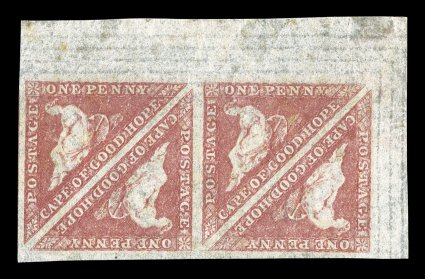
\includegraphics[width=.80\textwidth]{../cape-of-good-hope/SG5a.jpg}
\caption{35		S.G. 5a	S.G. 5a, 1858 1p Rose on cream toned paper, an extraordinarily handsome and choice corner sheet-margin block of four, huge margins all around, bright fresh color and impression, full o.g., couple of natural and trivial paper wrinkles, extremely fine; one of the finest quality mint multiples available; 1986 BPA certificate; ex-Sir Maxwell Joseph, Melat, "Salisbury" and Indhusophon (Scott 3).  Est. \$4,000-5,000 
SOLD for \$13,000.00}
\end{figure}


\begin{figure}[htbp]
\centering
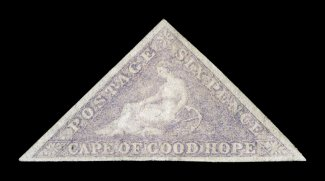
\includegraphics[width=.40\textwidth]{../cape-of-good-hope/SG7.jpg}
\caption{35		S.G. 5a	S.G. 5a, 1858 1p Rose on cream toned paper, an extraordinarily handsome and choice corner sheet-margin block of four, huge margins all around, bright fresh color and impression, full o.g., couple of natural and trivial paper wrinkles, extremely fine; one of the finest quality mint multiples available; 1986 BPA certificate; ex-Sir Maxwell Joseph, Melat, "Salisbury" and Indhusophon (Scott 3).  Est. \$4,000-5,000 
SOLD for \$13,000.00}
\end{figure}


\begin{figure}[htbp]
\centering
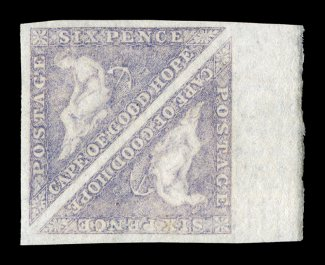
\includegraphics[width=.50\textwidth]{../cape-of-good-hope/SG7b.jpg}
\caption{37		S.G. 7b,	1858 6p Deep rose lilac on white paper, a gem mint marginal pair, featuring large to huge margins all around and lovely rich color, wonderfully fresh overall, nearly full o.g., extremely fine; a magnificent quality pair of a very scarce stamp; ex-West, Schofield, Huston, "Salisbury" and Indhusophon (Scott \#5a).  Est. \$4,000-5,000 
SOLD for \$10,500.00 gross}
\end{figure}
              